\documentclass[12pt,a4paper, spanish]{article}
\usepackage[spanish]{babel}
\usepackage[utf8]{inputenc}
\usepackage{setspace}
\usepackage[
  pdftex,
  pdfauthor={--- Arturo Vidal Peña & Javier Melero Deza ---},
  pdftitle={--- Práctica RESTful 2018/2019 ---},
  hidelinks]{hyperref}

% --- IMAGES ---
\usepackage[pdftex]{graphicx}
\usepackage{subfigure}
\usepackage{graphicx}
\usepackage{float}
\usepackage[usenames,dvipsnames]{color}
\DeclareGraphicsExtensions{.png,.jpg,.pdf,.mps,.gif,.bmp}
% --- IMAGES ---

% --- MARGIN DIMENSIONS ---
\frenchspacing \addtolength{\hoffset}{-1.5cm}
\addtolength{\textwidth}{3cm} \addtolength{\voffset}{-2.5cm}
\addtolength{\textheight}{4cm}
\setlength{\headheight}{15pt}
% --- MARGIN DIMENSIONS ---

% --- TITLE DATA ---
\title{\textbf{Práctica RESTful} \\
       \textsc{Sistemas Orientados a Servicios} \\
       \emph{DLSIIS}}
\author{\emph{Vidal Peña, Arturo}\\
        \emph{Melero Deza, Javier}}
\date{\underline{\today}}
% --- TITLE DATA ---

% --- TABLE OF CONTENTS' DOTS
\usepackage{tocloft}
\renewcommand{\cftsecleader}{\cftdotfill{\cftdotsep}}
% --- TABLE OF CONTENTS' DOTS

% --- DOCUMENT ---
\begin{document}

% --- TITLE ---
\maketitle
\thispagestyle{empty}
\pagenumbering{gobble}
\renewcommand*\contentsname{Índice de contenidos}
\tableofcontents
\pagebreak
% --- TITLE ---

\pagenumbering{arabic}

\section{Resumen del diseño del servicio}
La arquitectura de la aplicación consta de una base de datos simple formada por 4 tablas:

\begin{itemize}
	\item Usuarios
	\item Mensajes
	\item Privados
	\item Amistad
\end{itemize}

Posteriormente se programan los recursos, modelos y servicios necesarios para cumplir con las especificaciones pedidas utilizando Jersey Restful. \newline

Dicho servidor se ejecuta sobre Apache Maven en \textit{localhost} con puerto 8080. Internamente, la aplicación proporciona servicios desde la clase UserResource utilizando el resto de clases con las estructuras adecuadas para la conexión con la base de datos y posteriormente su conversión a JSON o XML.

\newpage
\section{Capturas de la ejecución en un cliente REST (Postman)}
Hay que poner detalles tanto de la invocación como del resultado de la operación.

\begin{figure}[H]
	\centering
	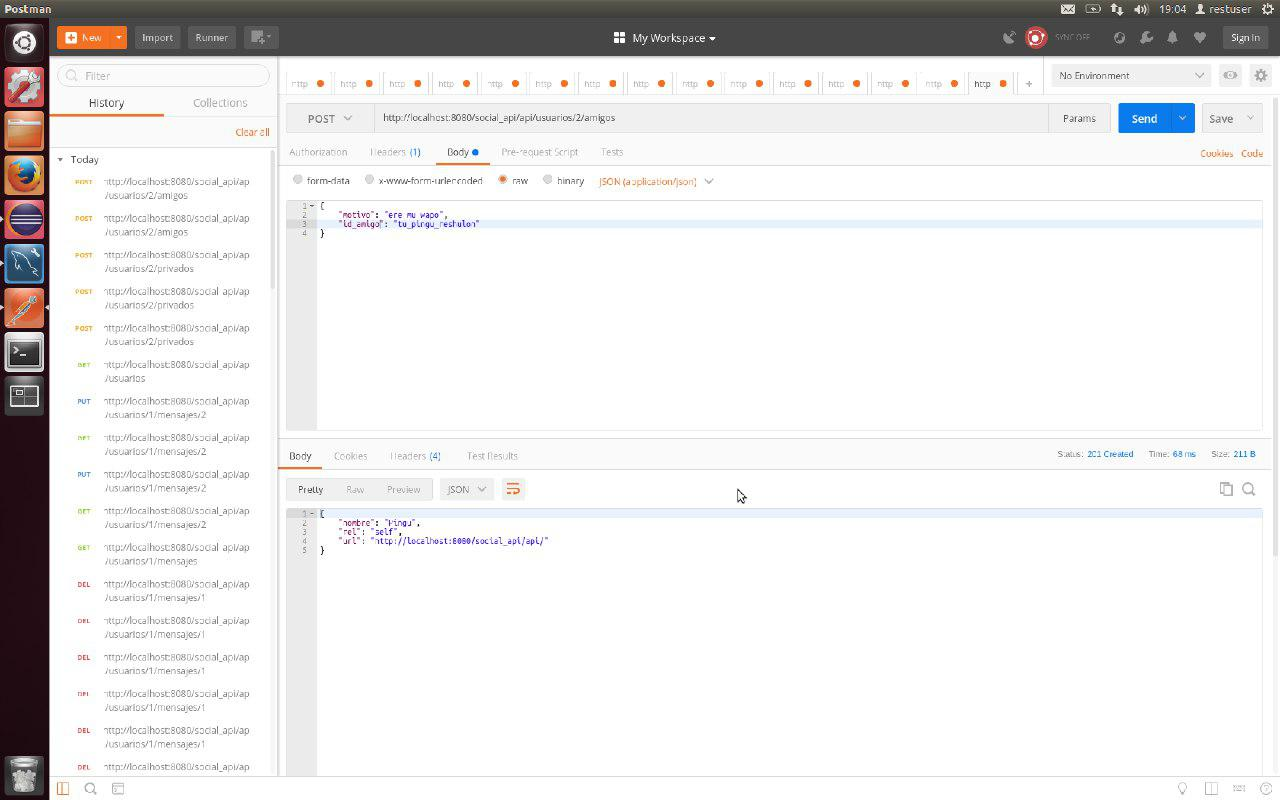
\includegraphics[width=0.75\textwidth]{images/captura1.jpg}
	\caption{Método POST para insertar un amigo en el usuario con id 2.}
\end{figure}

\begin{figure}[H]
	\centering
	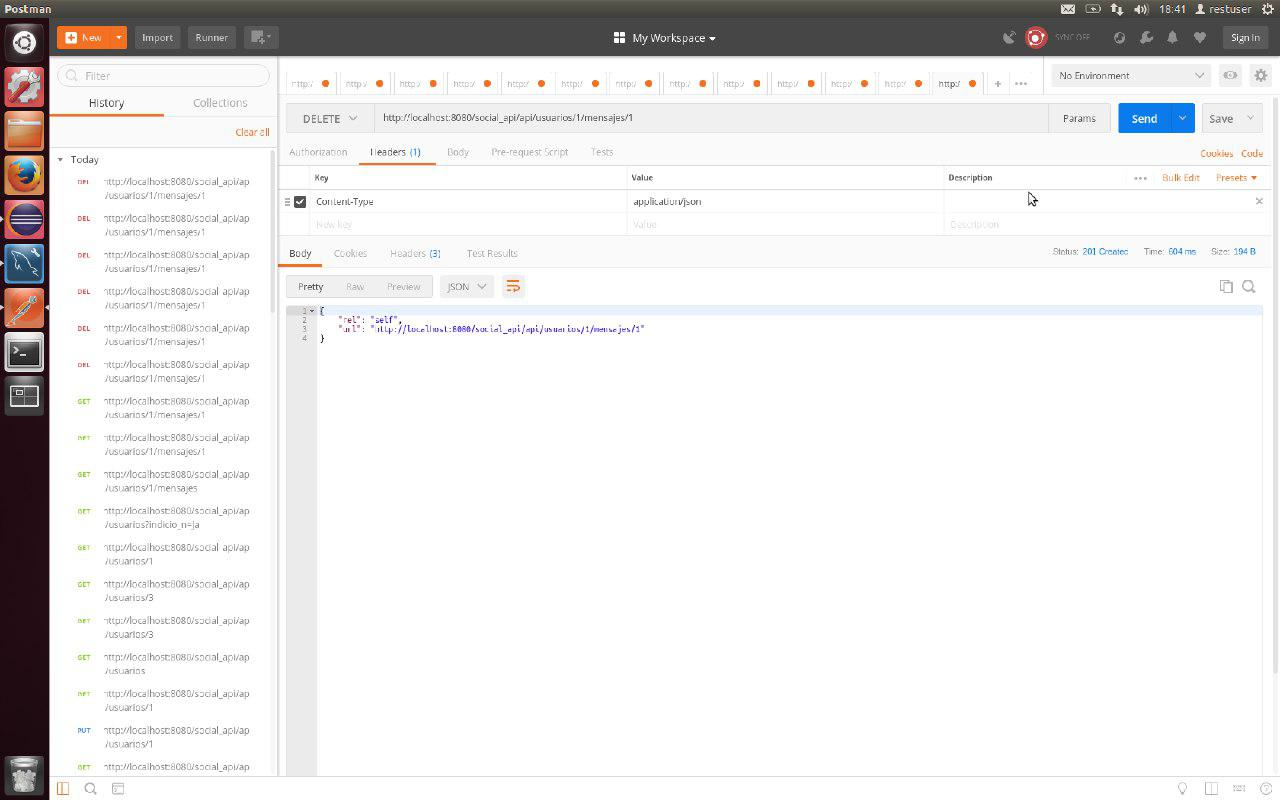
\includegraphics[width=0.75\textwidth]{images/captura2.jpg}
	\caption{Método DELETE para borrar un mensaje del usuario con id 1.}
\end{figure}

\begin{figure}[H]
	\centering
	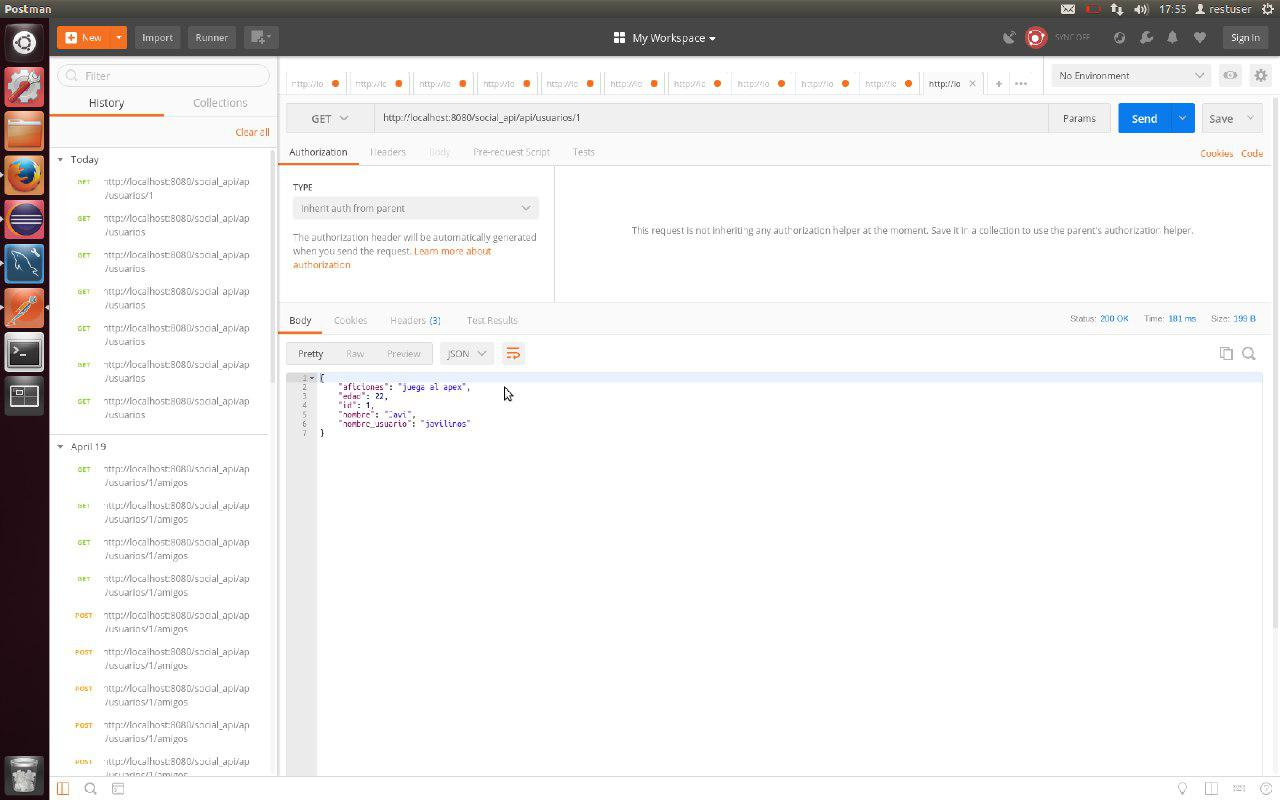
\includegraphics[width=0.75\textwidth]{images/captura3.jpg}
	\caption{Método GET para obtener la información del usuario con id 1.}
\end{figure}

\begin{figure}[H]
	\centering
	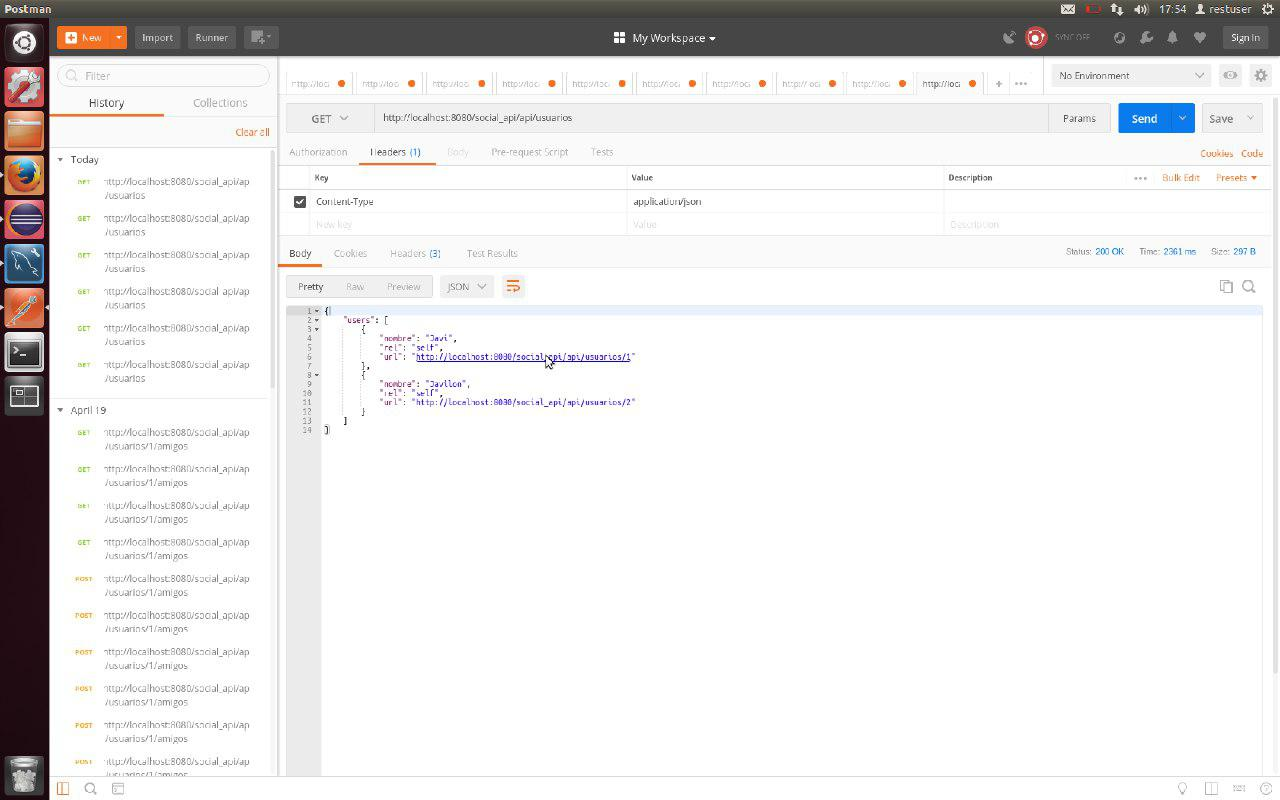
\includegraphics[width=0.75\textwidth]{images/captura4.jpg}
	\caption{Método GET para obtener la información de todos los usuarios.}
\end{figure}

%\begin{figure}[H]
%	\centering
%	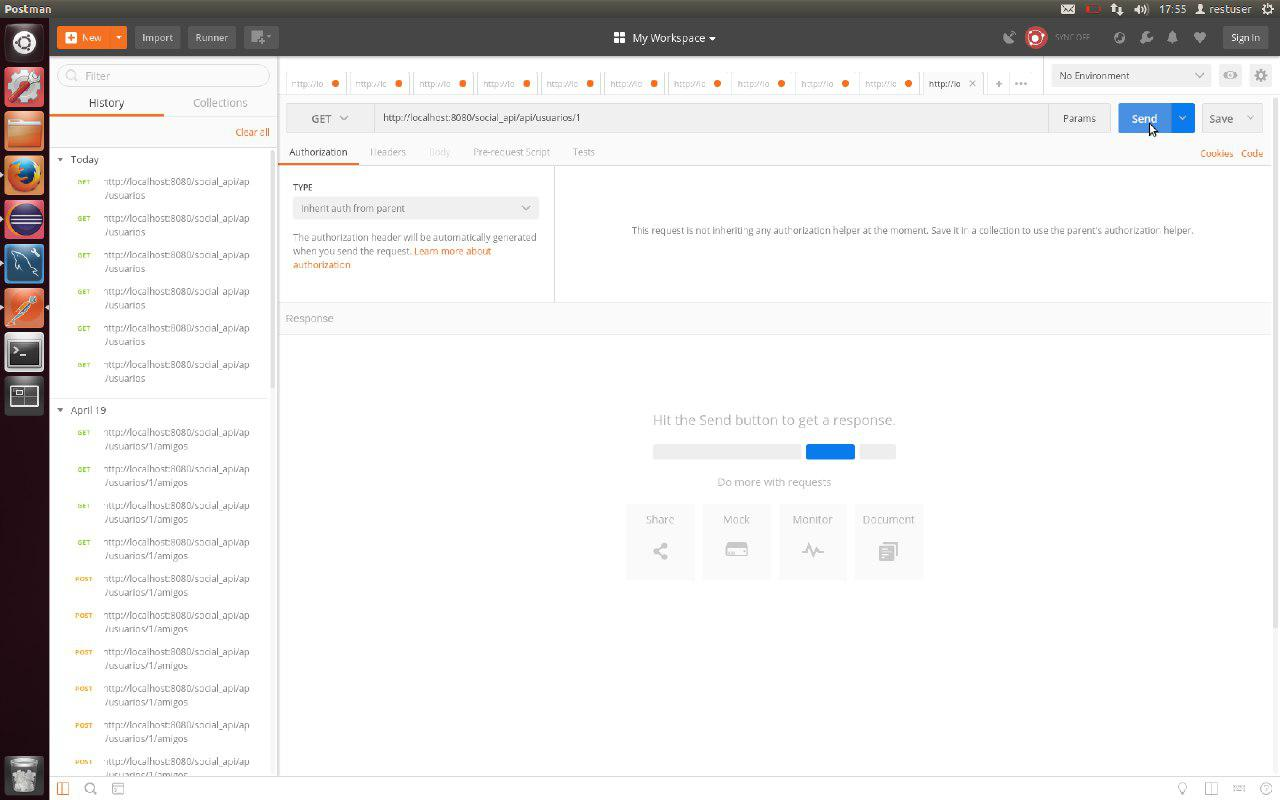
\includegraphics[width=0.75\textwidth]{images/captura5.jpg}
%	\caption{Método GET}
%\end{figure}

\begin{figure}[H]
	\centering
	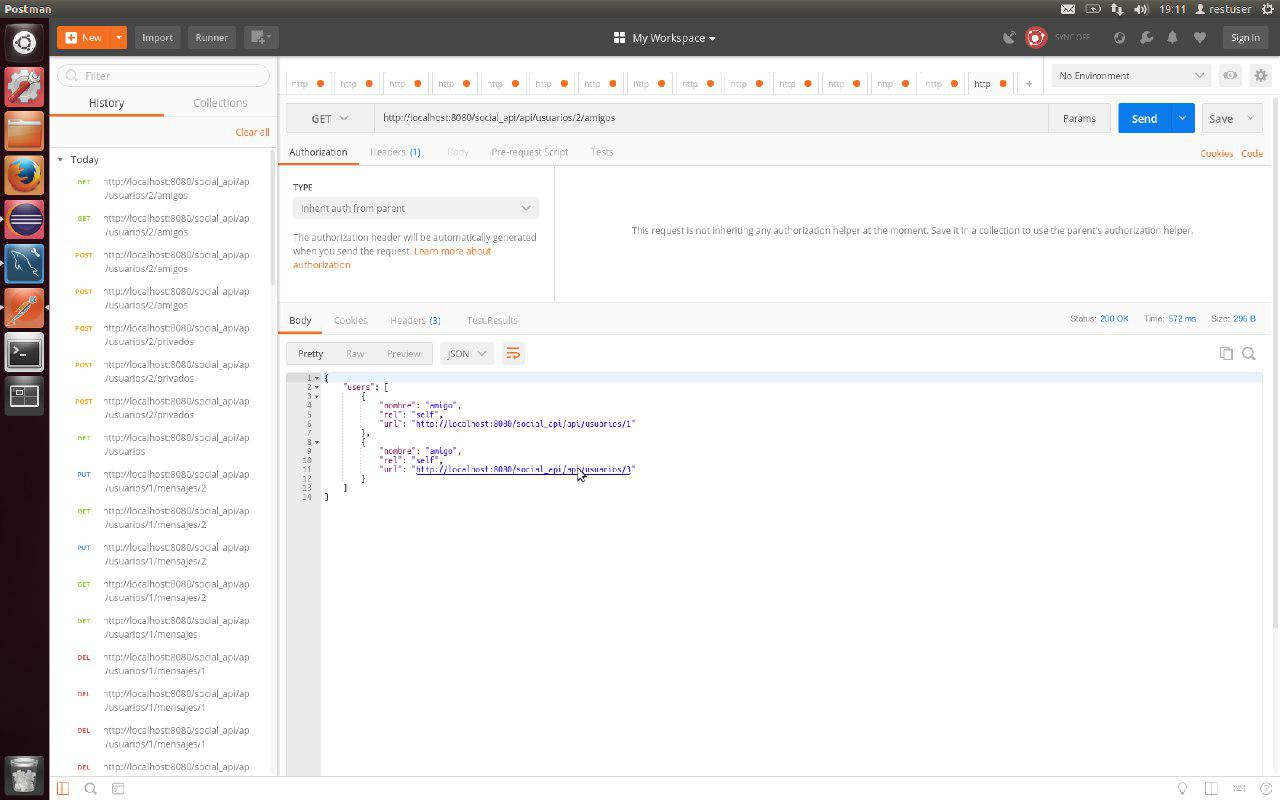
\includegraphics[width=0.75\textwidth]{images/captura6.jpg}
	\caption{Método GET para obtener los amigos del usuario con id 2.}
\end{figure}

\begin{figure}[H]
	\centering
	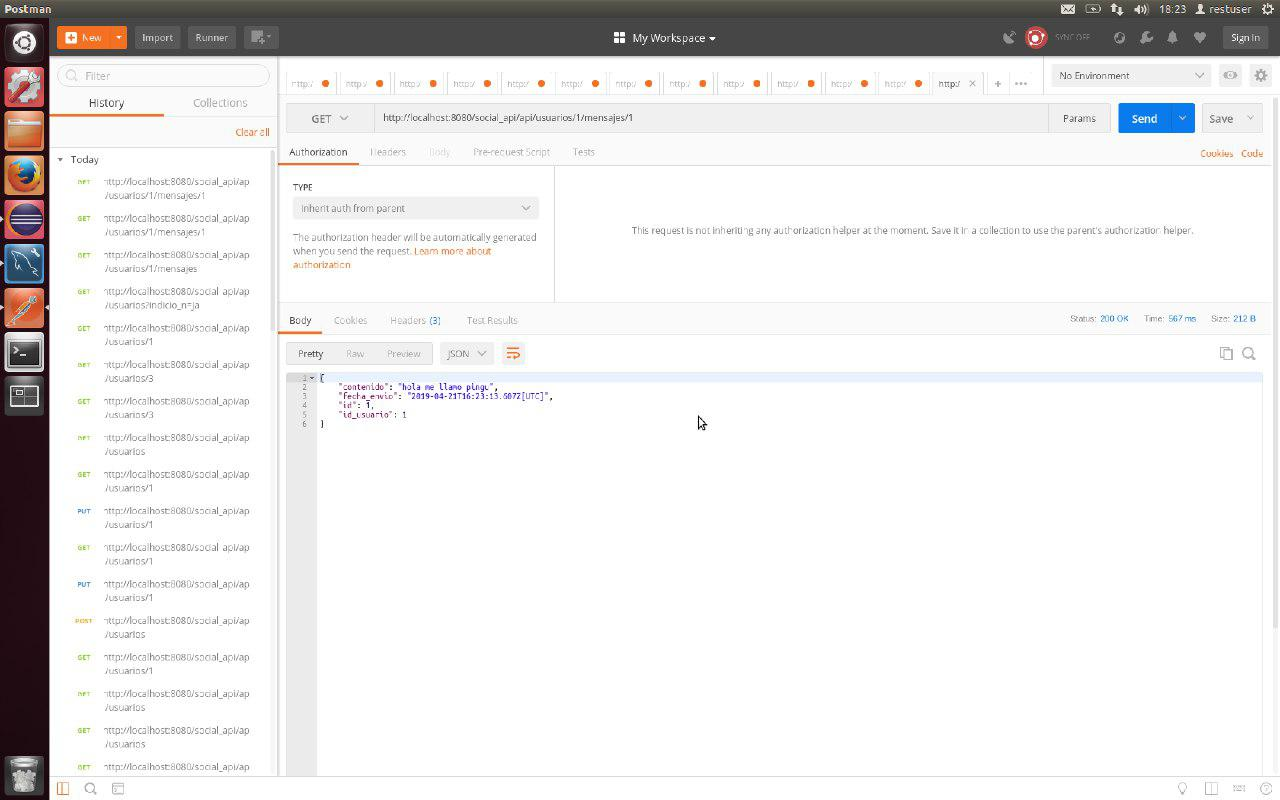
\includegraphics[width=0.75\textwidth]{images/captura7.jpg}
	\caption{Método GET para obtener la información del mensaje con id 1 del usuario con id 1.}
\end{figure}

\begin{figure}[H]
	\centering
	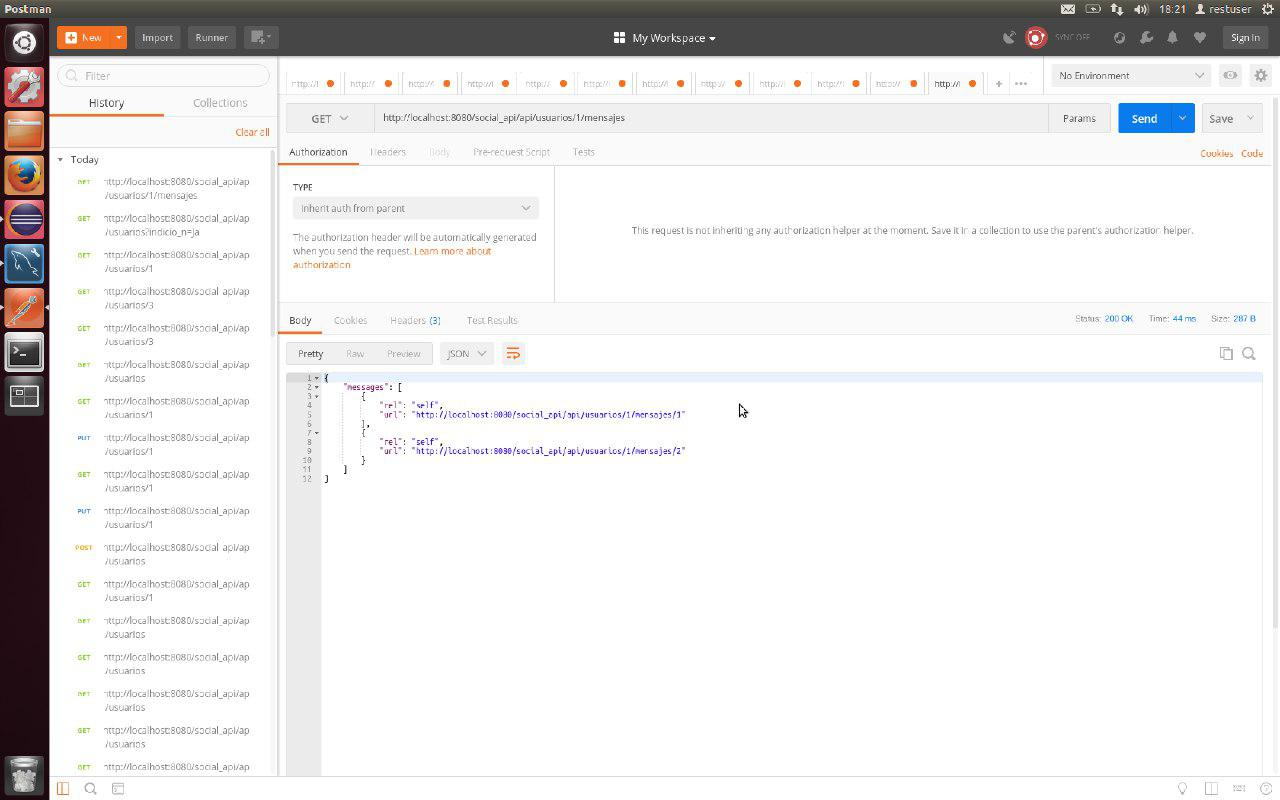
\includegraphics[width=0.75\textwidth]{images/captura8.jpg}
	\caption{Método GET para obtener los mensajes del usuario con id 1.}
\end{figure}

\begin{figure}[H]
	\centering
	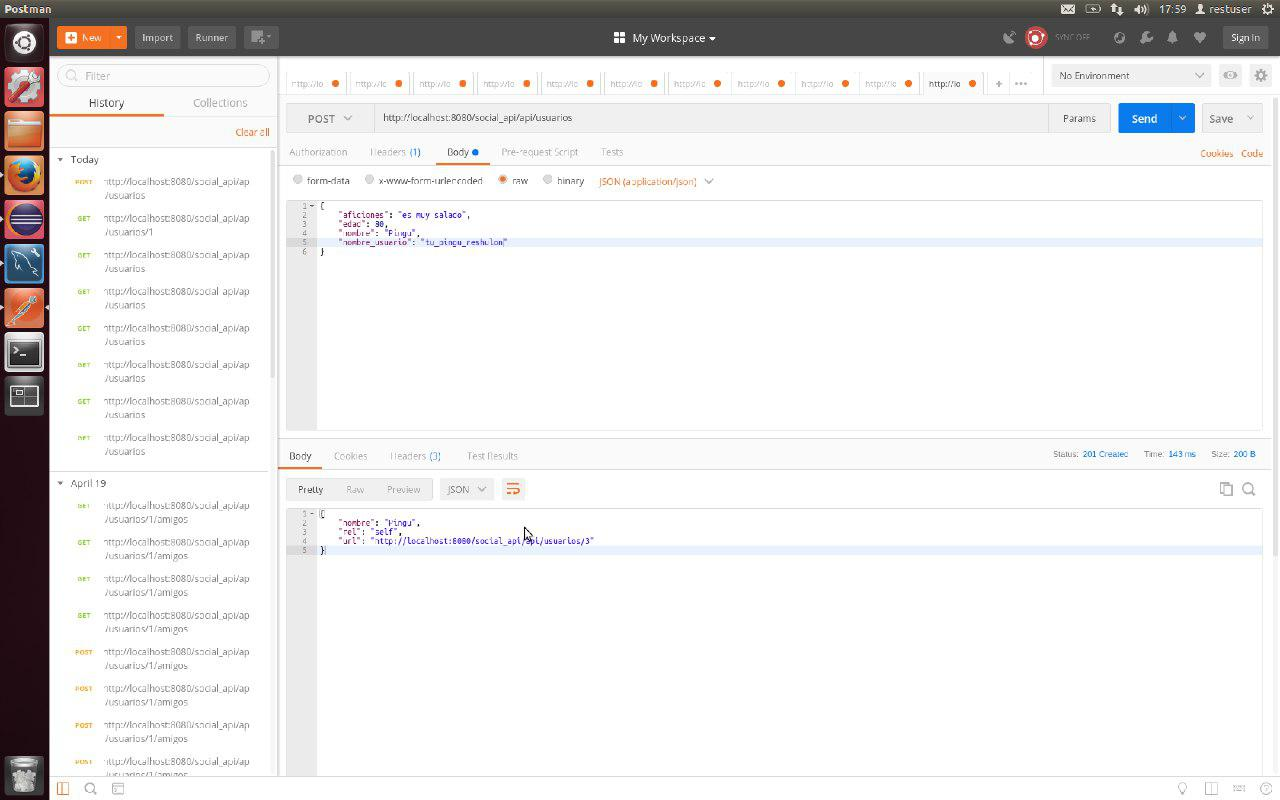
\includegraphics[width=0.75\textwidth]{images/captura9.jpg}
	\caption{Método POST para añadir un nuevo usuario con id 3.}
\end{figure}

\begin{figure}[H]
	\centering
	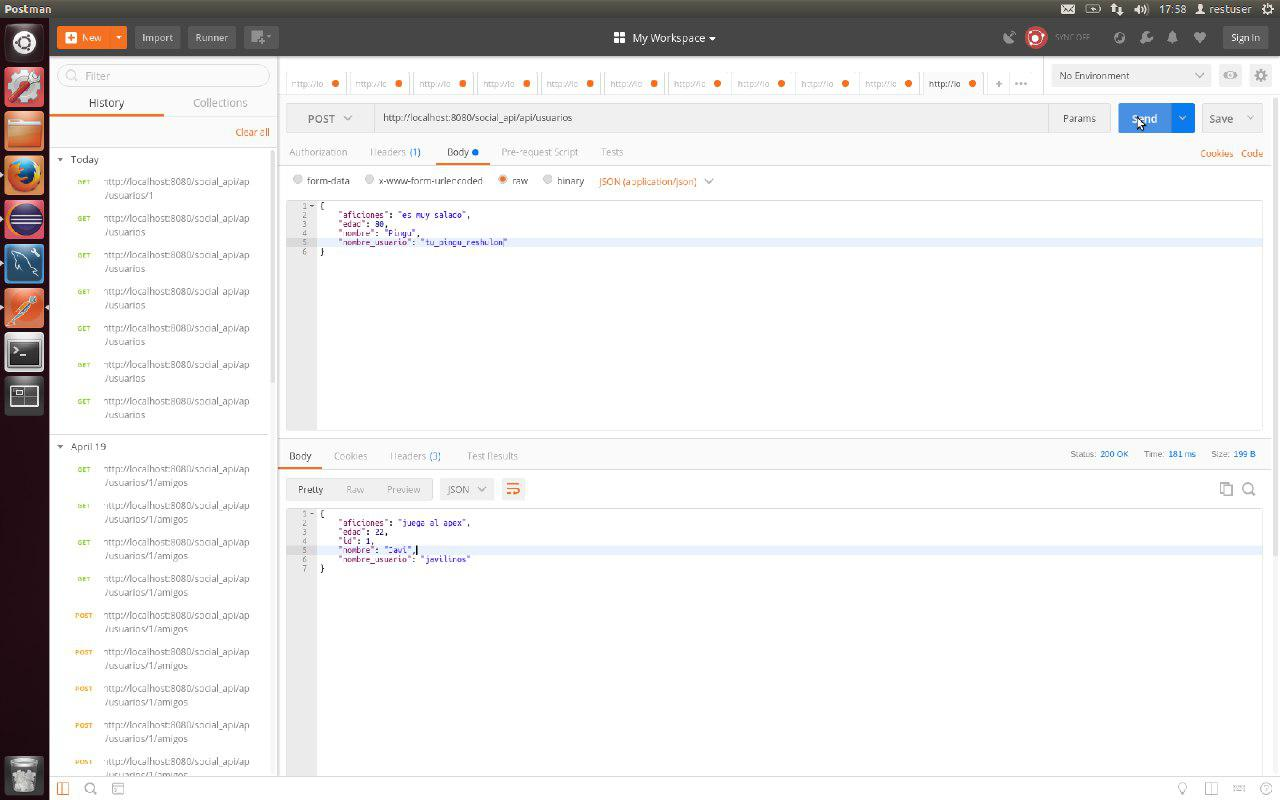
\includegraphics[width=0.75\textwidth]{images/captura10.jpg}
	\caption{Método POST para añadir un nuevo usuario con id 1.}
\end{figure}

\begin{figure}[H]
	\centering
	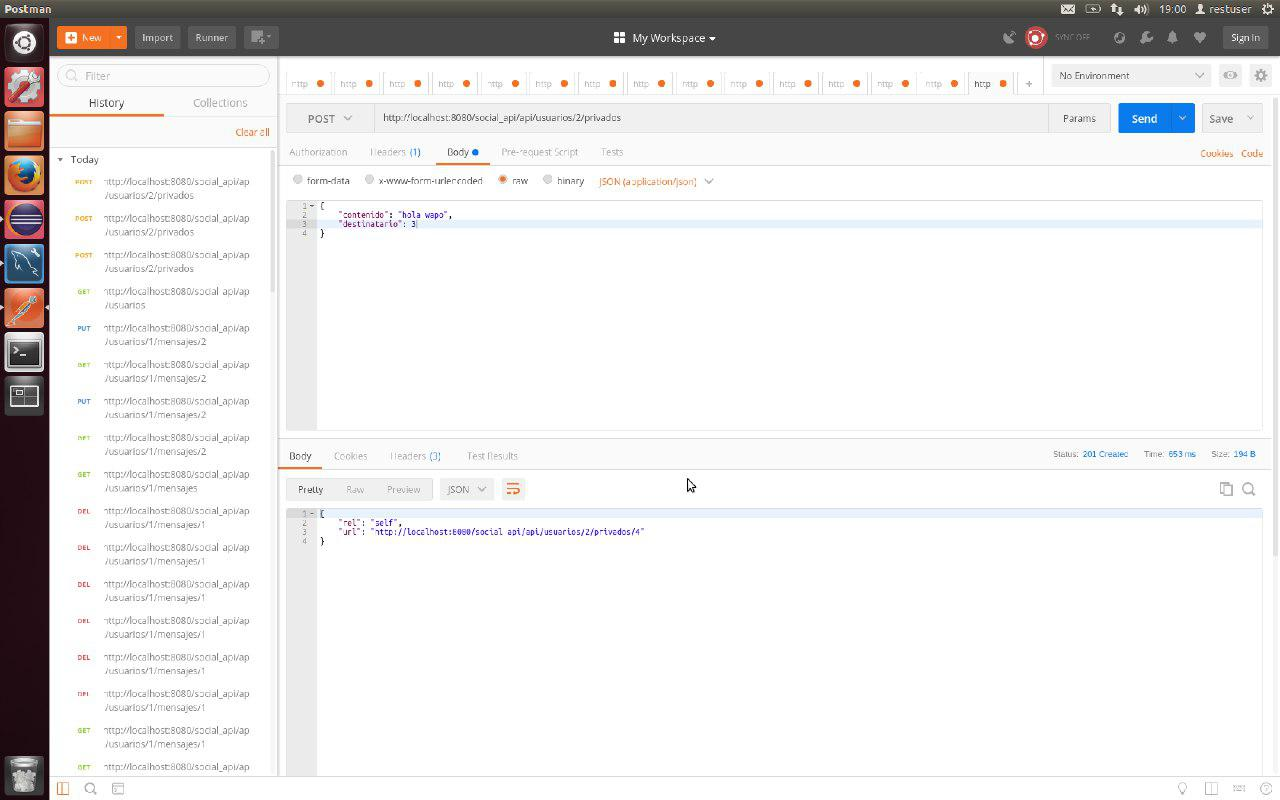
\includegraphics[width=0.75\textwidth]{images/captura11.jpg}
	\caption{Método POST para añadir un nuevo mensaje privado desde el usuario con id 2 al usuario con id 3.}
\end{figure}

\begin{figure}[H]
	\centering
	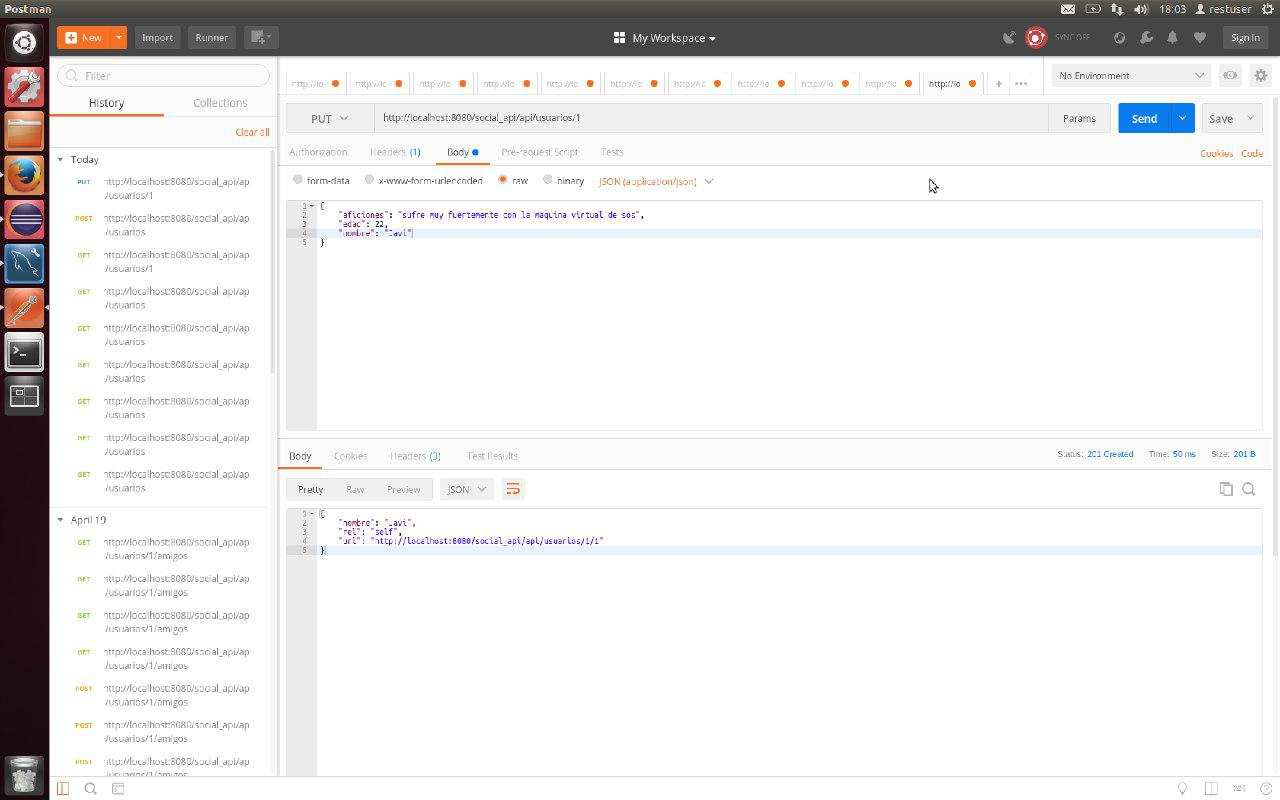
\includegraphics[width=0.75\textwidth]{images/captura12.jpg}
	\caption{Método PUT para modificar datos pertenecientes al usuario con id 1.}
\end{figure}

\begin{figure}[H]
	\centering
	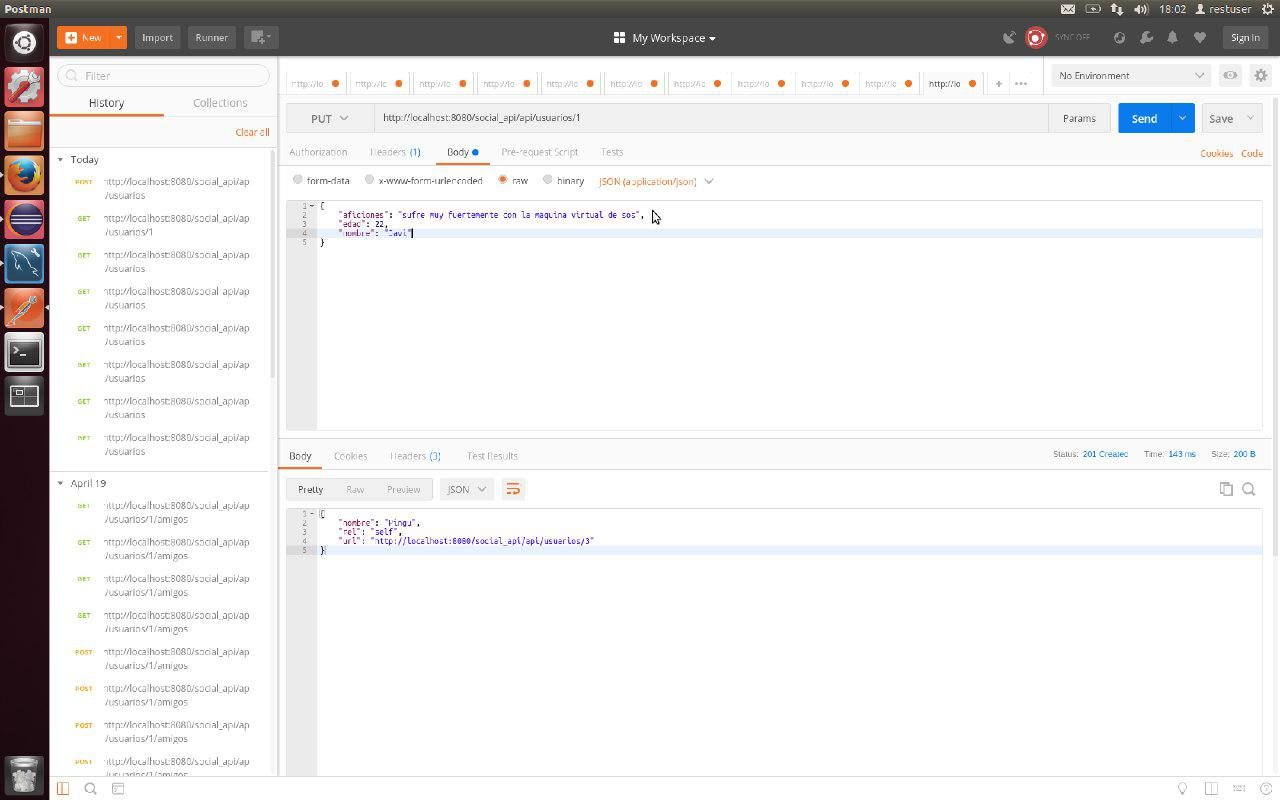
\includegraphics[width=0.75\textwidth]{images/captura13.jpg}
	\caption{Método PUT para modificar datos pertenecientes al usuario con id 1.}
\end{figure}

\begin{figure}[H]
	\centering
	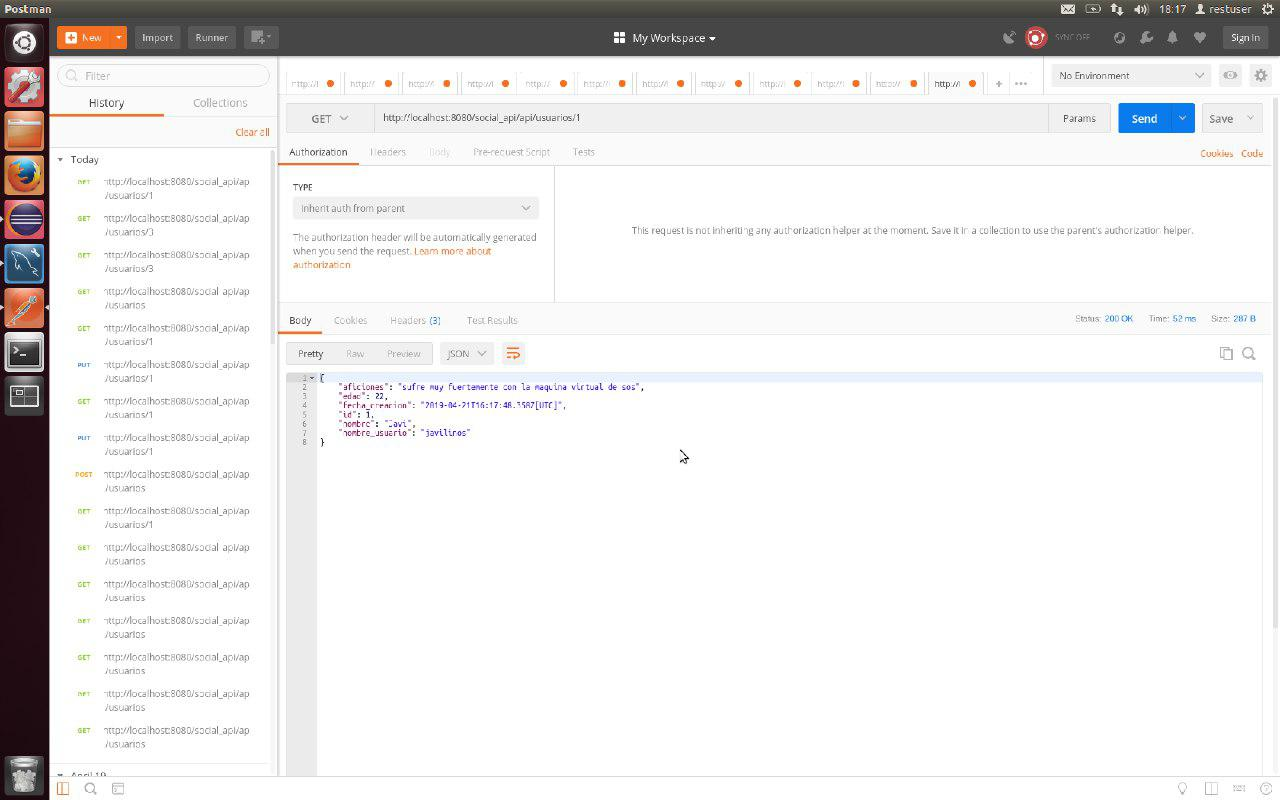
\includegraphics[width=0.75\textwidth]{images/captura14.jpg}
	\caption{Método GET para obtener la información del usuario con id 1.}
\end{figure}

\begin{figure}[H]
	\centering
	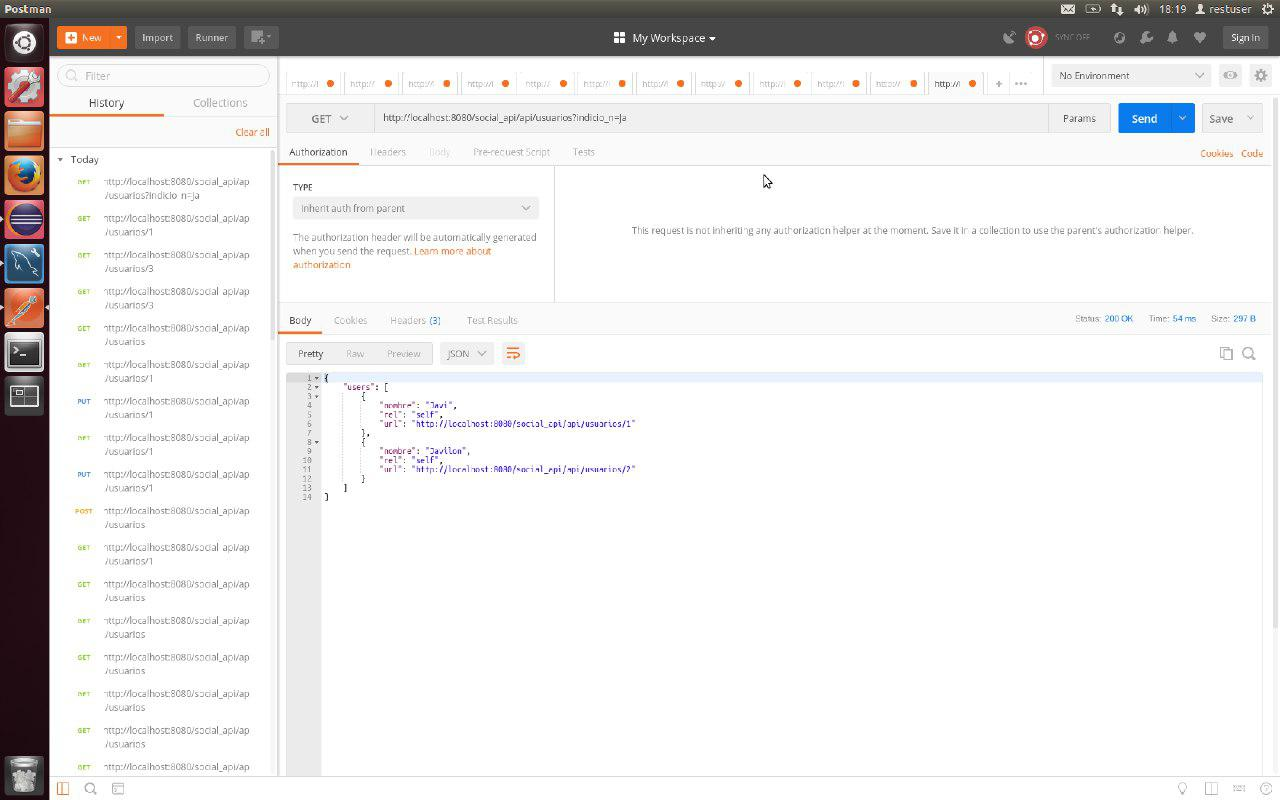
\includegraphics[width=0.75\textwidth]{images/captura15.jpg}
	\caption{Método GET para obtener los usuarios cuyo nombre empieza por "Ja".}
\end{figure}

\begin{figure}[H]
	\centering
	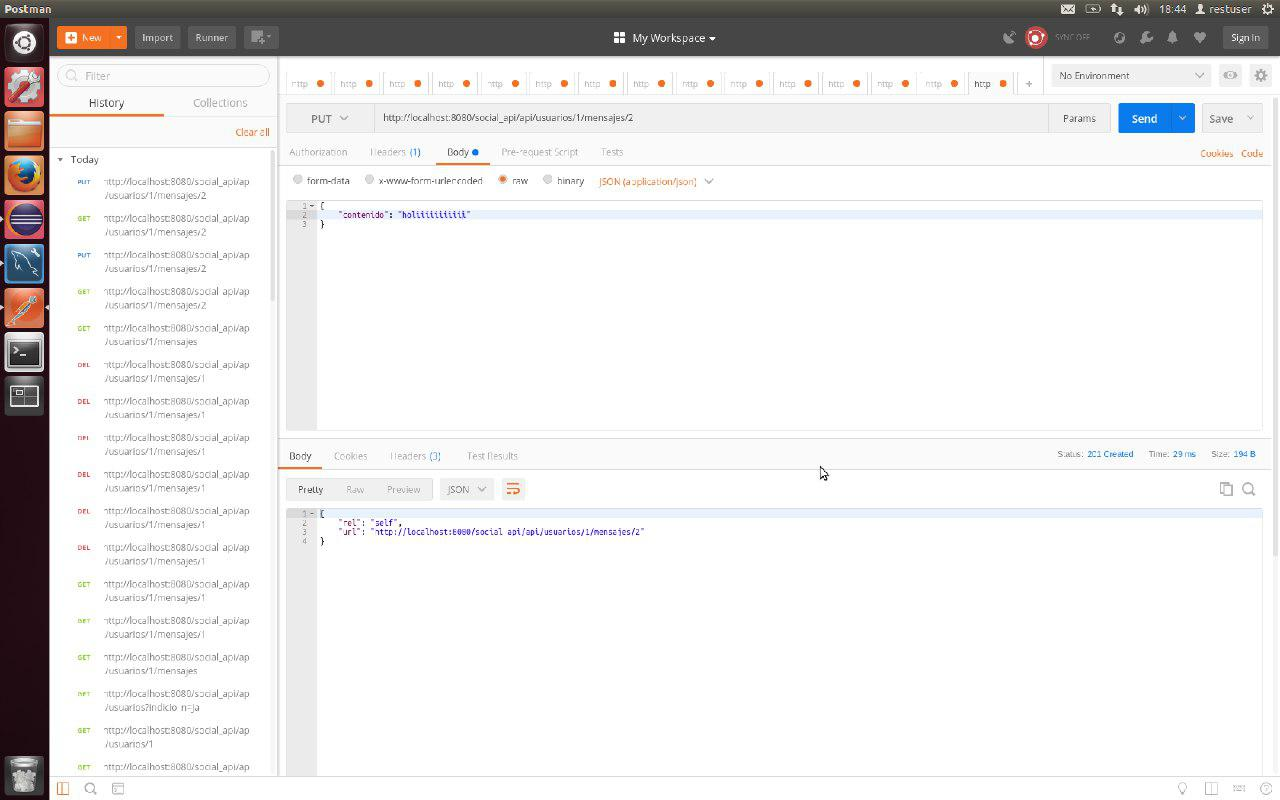
\includegraphics[width=0.75\textwidth]{images/captura16.jpg}
	\caption{Método PUT para modificar el mensaje con id 2 de la página del usuario con id 1.}
\end{figure}

\begin{figure}[H]
	\centering
	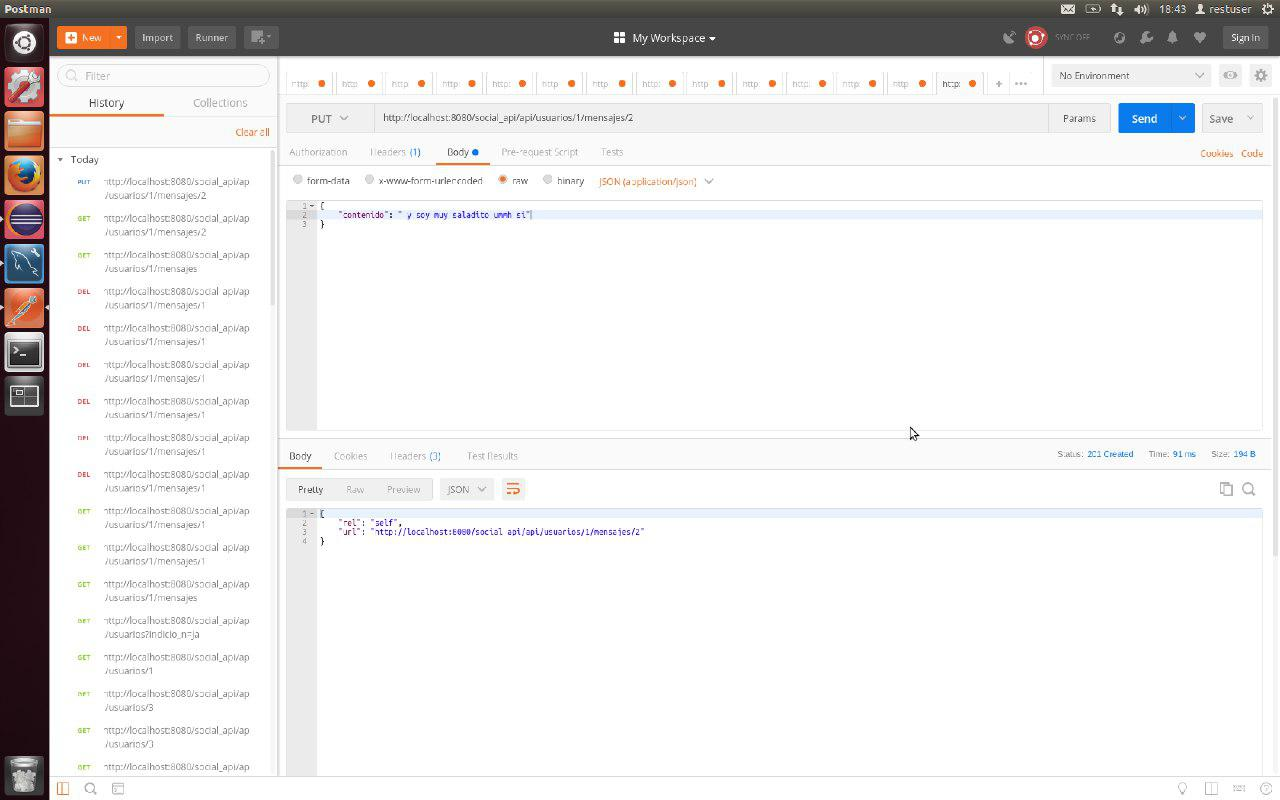
\includegraphics[width=0.75\textwidth]{images/captura17.jpg}
	\caption{Método PUT para modificar el mensaje con id 2 de la página del usuario con id 1.}
\end{figure}

\begin{figure}[H]
	\centering
	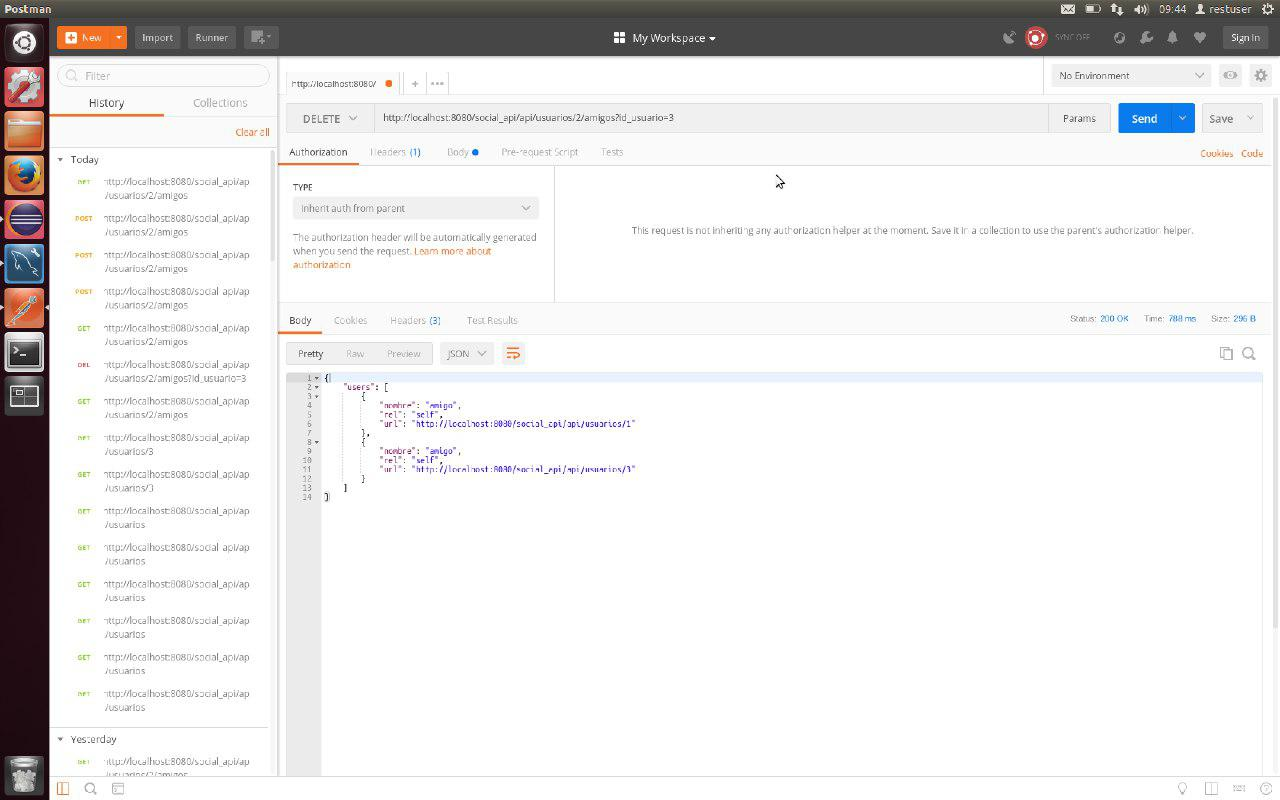
\includegraphics[width=0.75\textwidth]{images/captura18.jpg}
	\caption{Método DELETE para eliminar al usuario con id 3 de la lista de amigos del usuario con id 2.}
\end{figure}

%\begin{figure}[H]
%	\centering
%	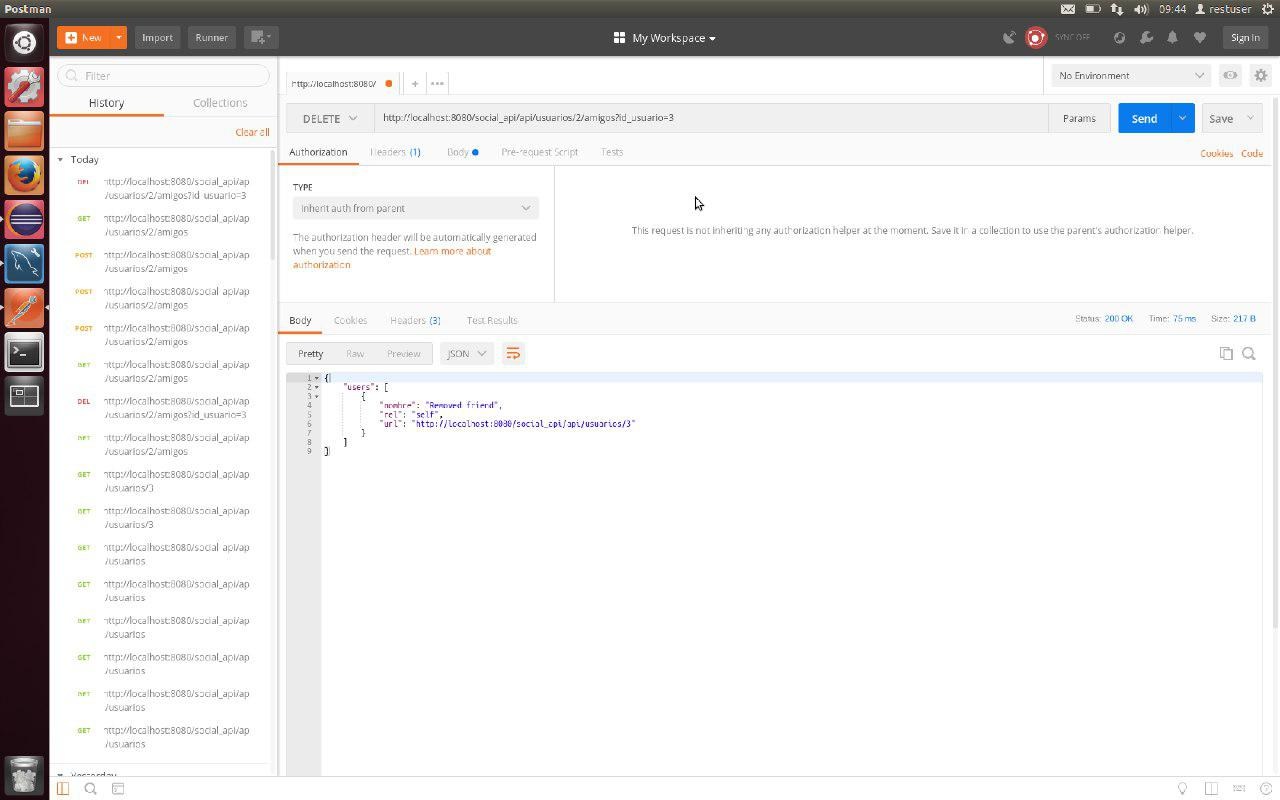
\includegraphics[width=0.75\textwidth]{images/captura19.jpg}
%	\caption{Método DELETE}
%\end{figure}

\begin{figure}[H]
	\centering
	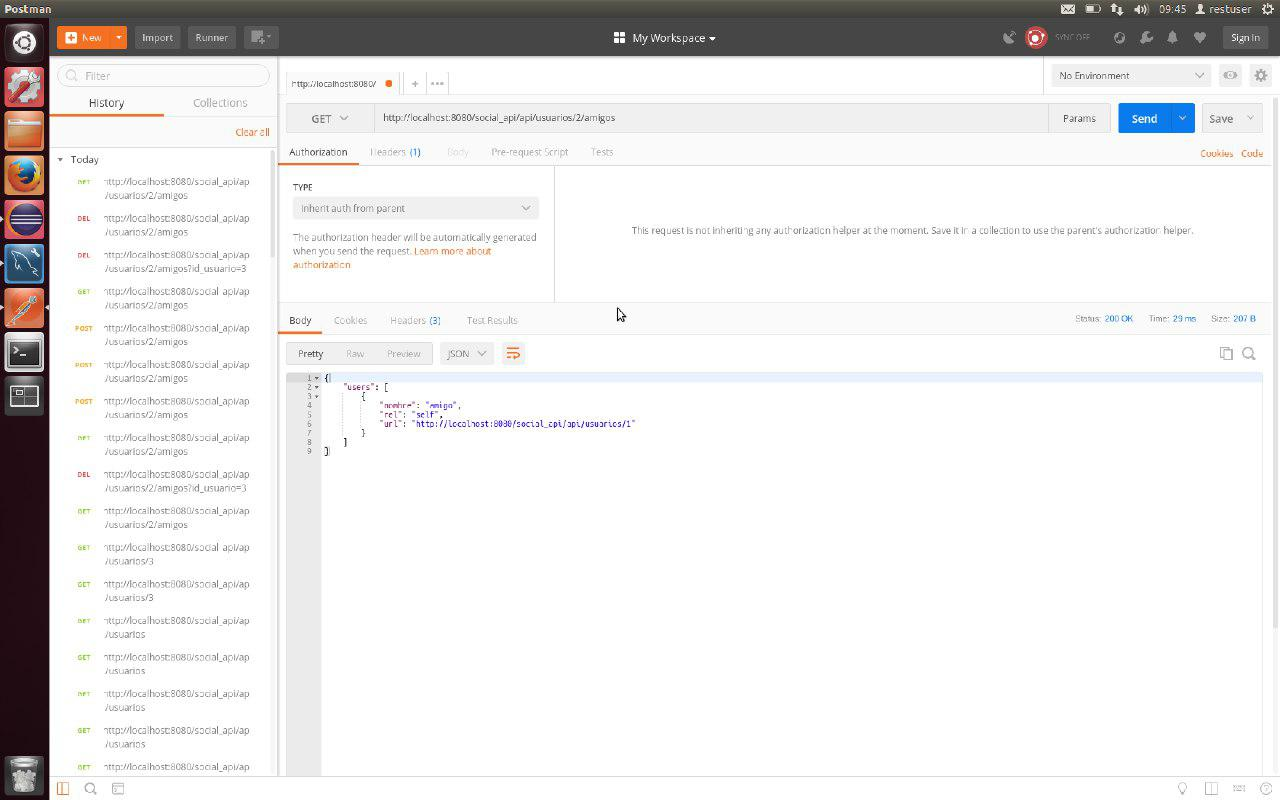
\includegraphics[width=0.75\textwidth]{images/captura20.jpg}
	\caption{Método GET para obtener la lista de amigos del usuario con id 2.}
\end{figure}

\begin{figure}[H]
	\centering
	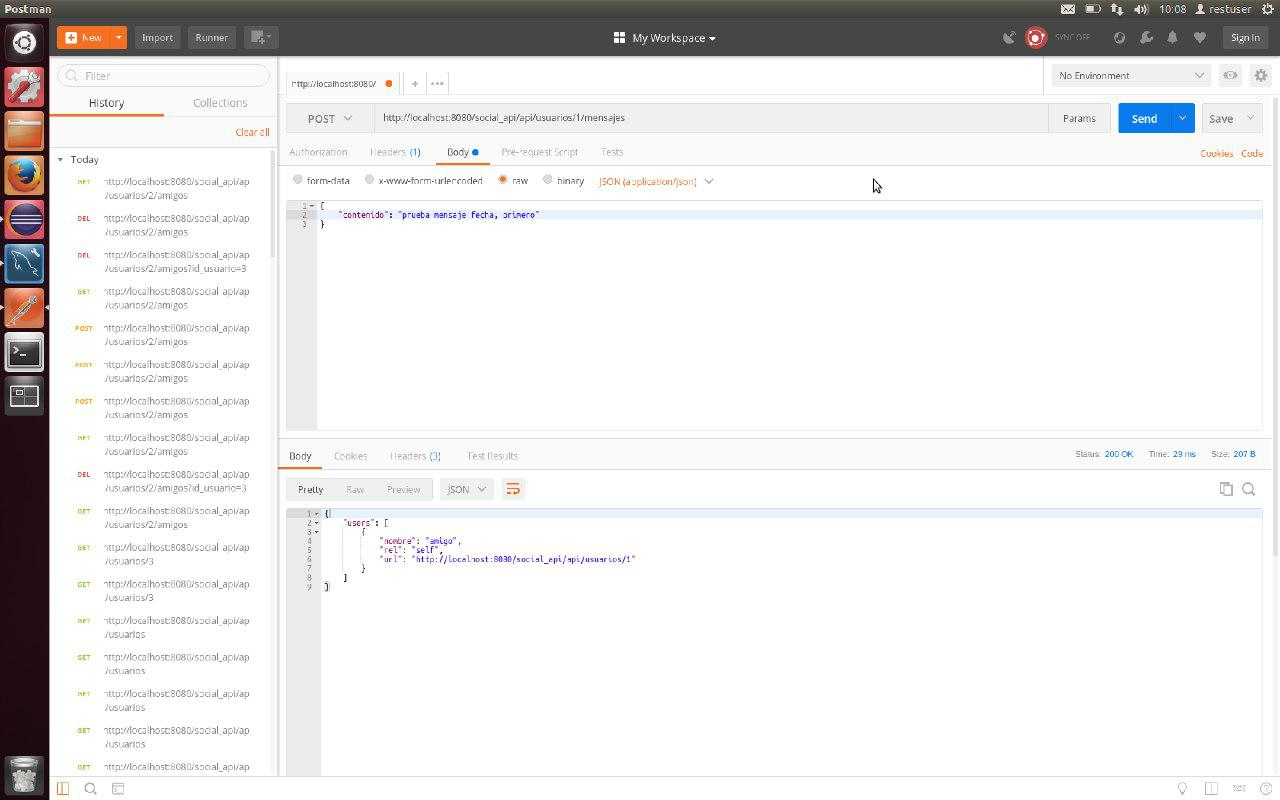
\includegraphics[width=0.75\textwidth]{images/captura21.jpg}
	\caption{Método POST para añadir un mensaje en la página del usuario con id 1.}
\end{figure}

\begin{figure}[H]
	\centering
	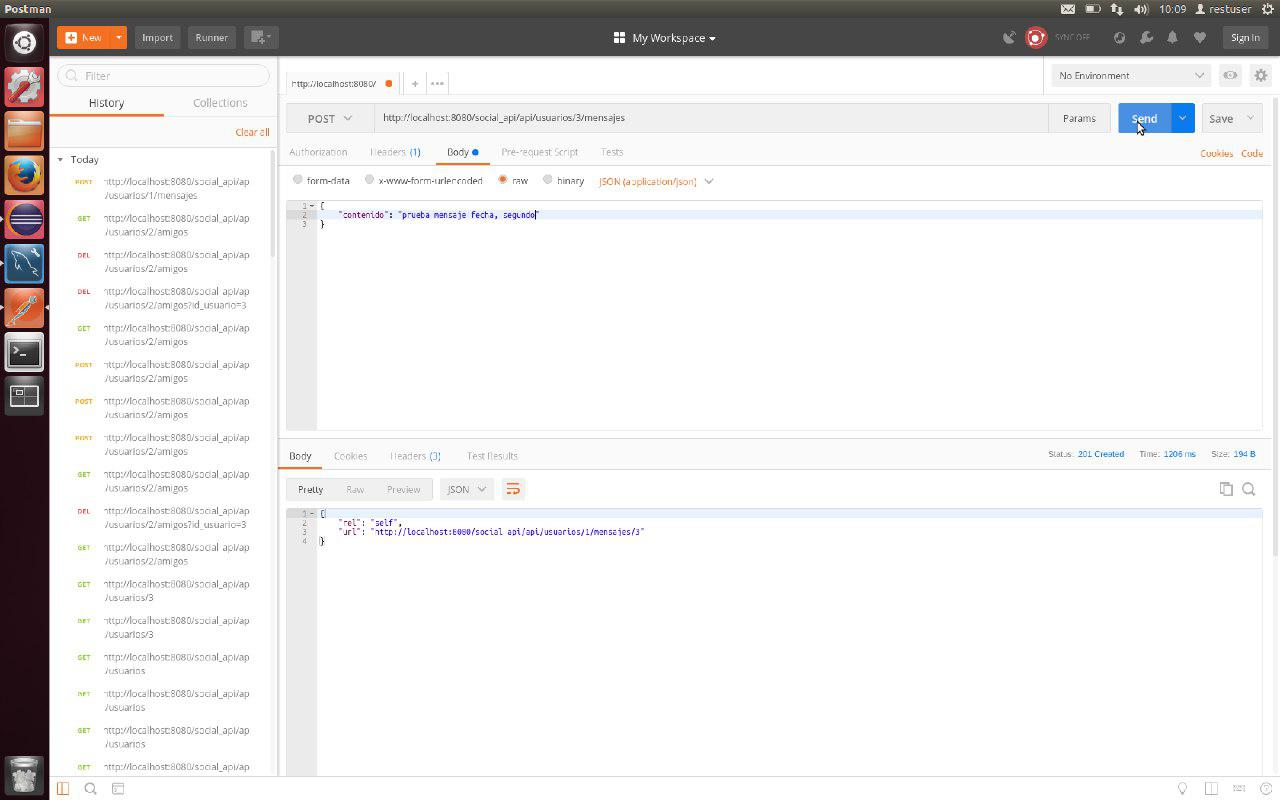
\includegraphics[width=0.75\textwidth]{images/captura22.jpg}
	\caption{Método POST para añadir un mensaje en la página del usuario con id 3.}
\end{figure}

\begin{figure}[H]
	\centering
	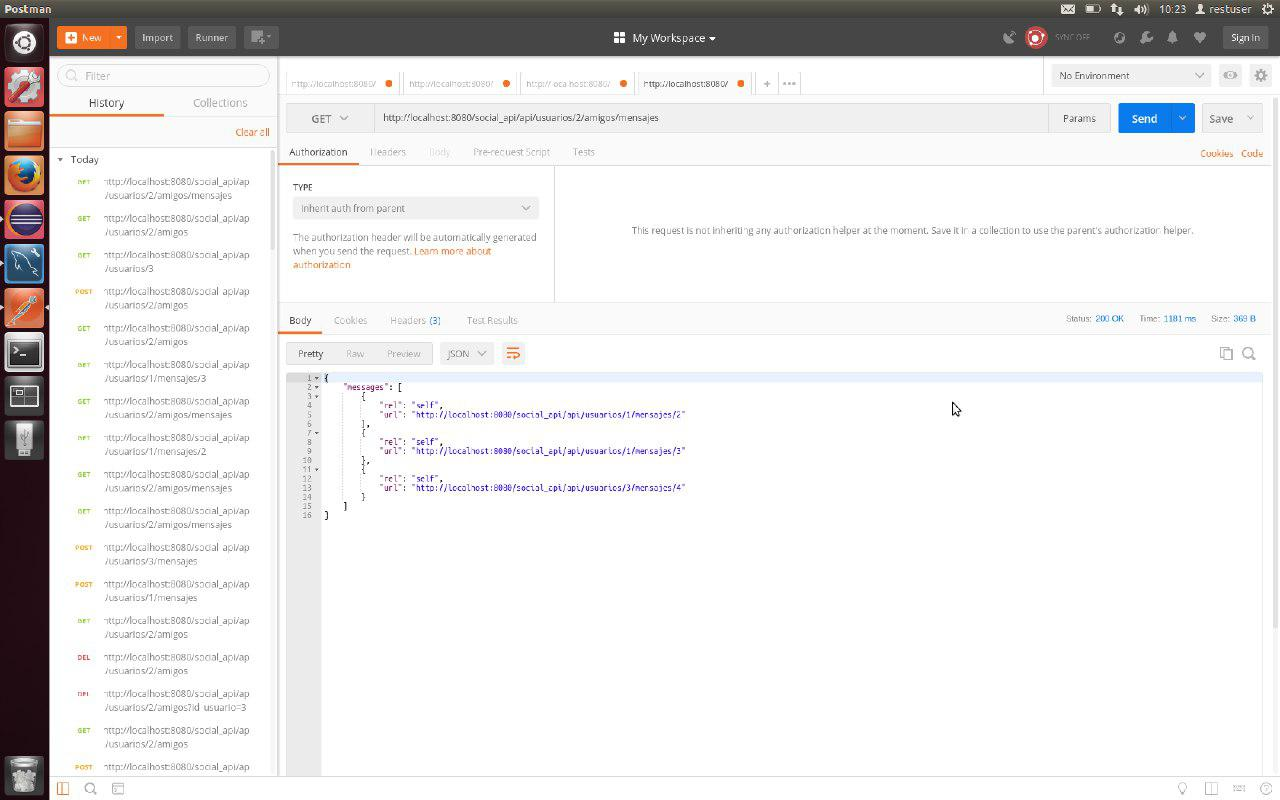
\includegraphics[width=0.75\textwidth]{images/captura23.jpg}
	\caption{Método GET para obtener los mensajes de amigos del usuario con id 2.}
\end{figure}

\begin{figure}[H]
	\centering
	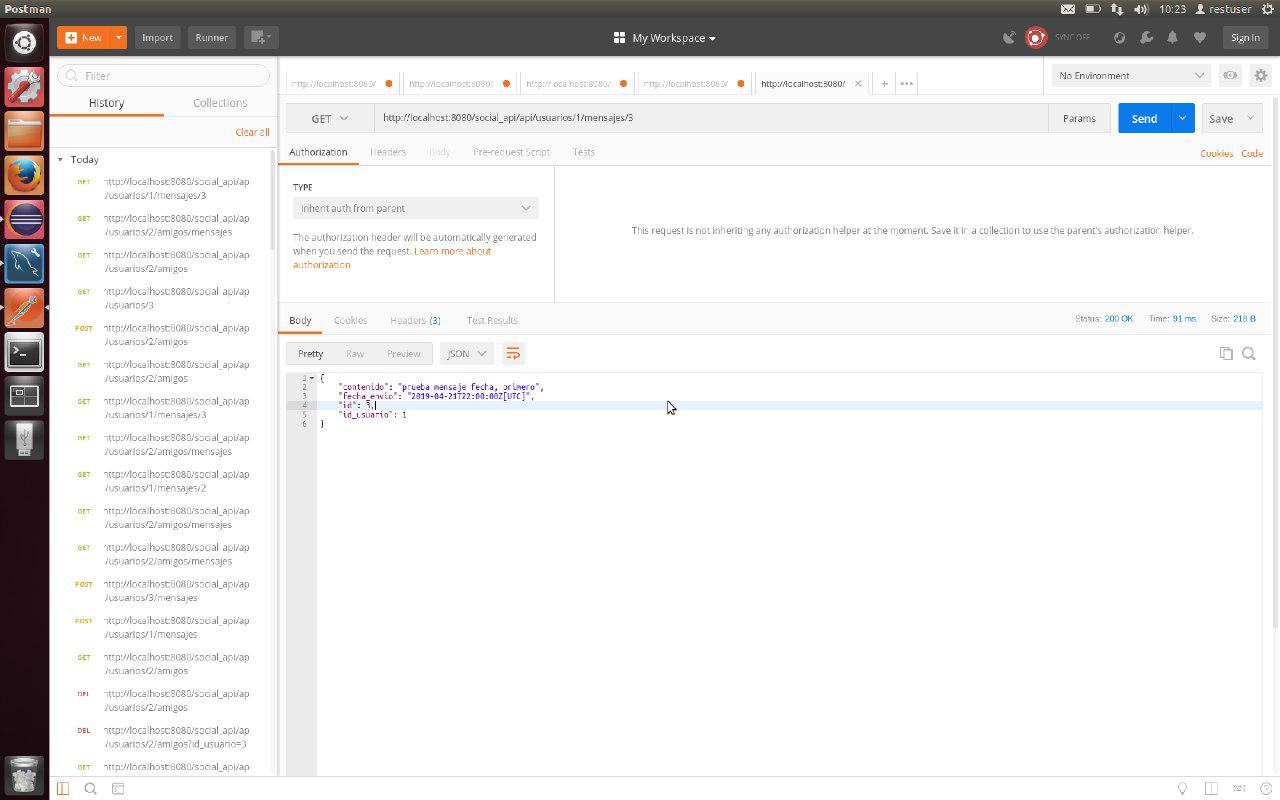
\includegraphics[width=0.75\textwidth]{images/captura24.jpg}
	\caption{Método GET para obtener el mensaje con id 3 del usuario con id 1.}
\end{figure}

\begin{figure}[H]
	\centering
	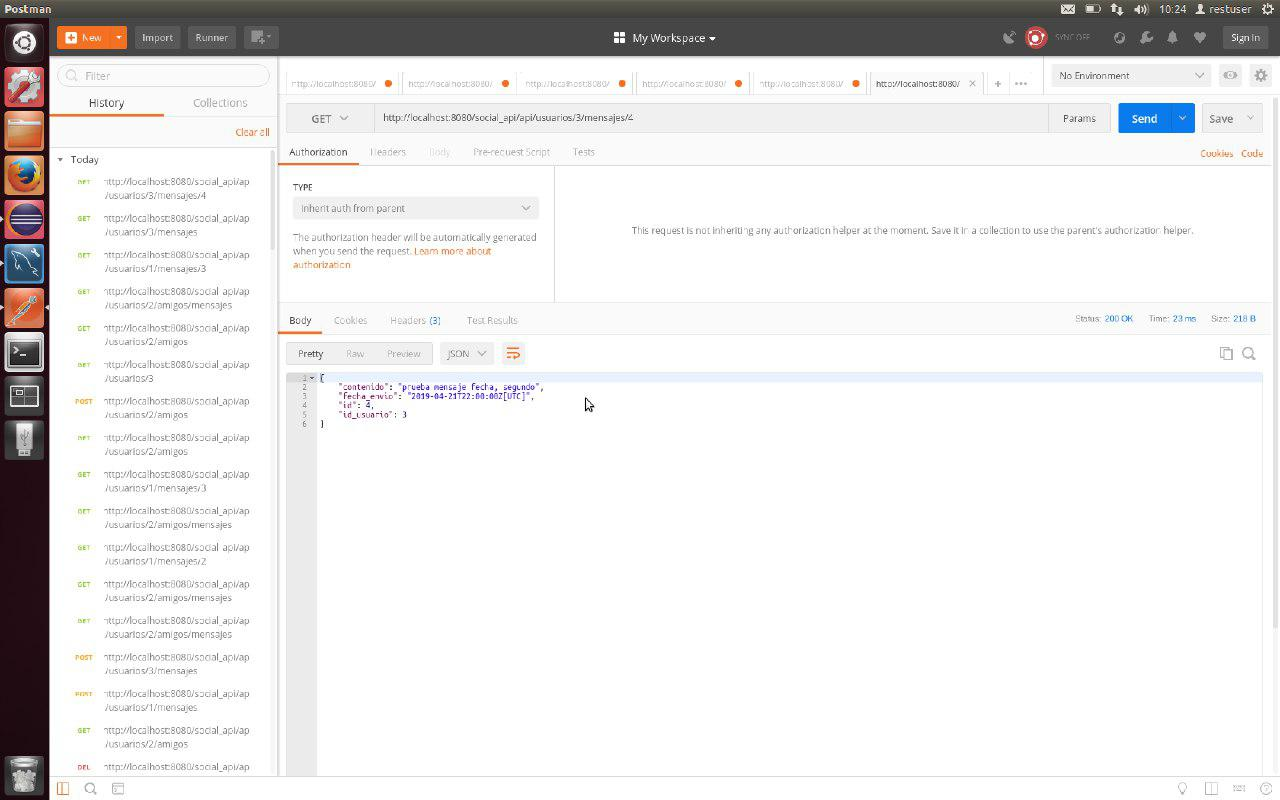
\includegraphics[width=0.75\textwidth]{images/captura25.jpg}
	\caption{Método GET para obtener el mensaje con id 4 del usuario con id 3.}
\end{figure}

\newpage
\section{ANEXO: Problemas encontrados}

Los fallos encontrados referentes a la Máquina virtual son:

\begin{itemize}
	\item Con la aplicación Postman, al probar los métodos HTTP.
	\item Con la aplicación Eclipse, que algunas veces no encontraba las URIs implementadas.
	\item Con la baja calidad de las capturas de pantalla del SO utilizado (probablemente por la antigüedad del mismo).
\end{itemize} 

\begin{figure}[H]
	\centering
	\subfigure{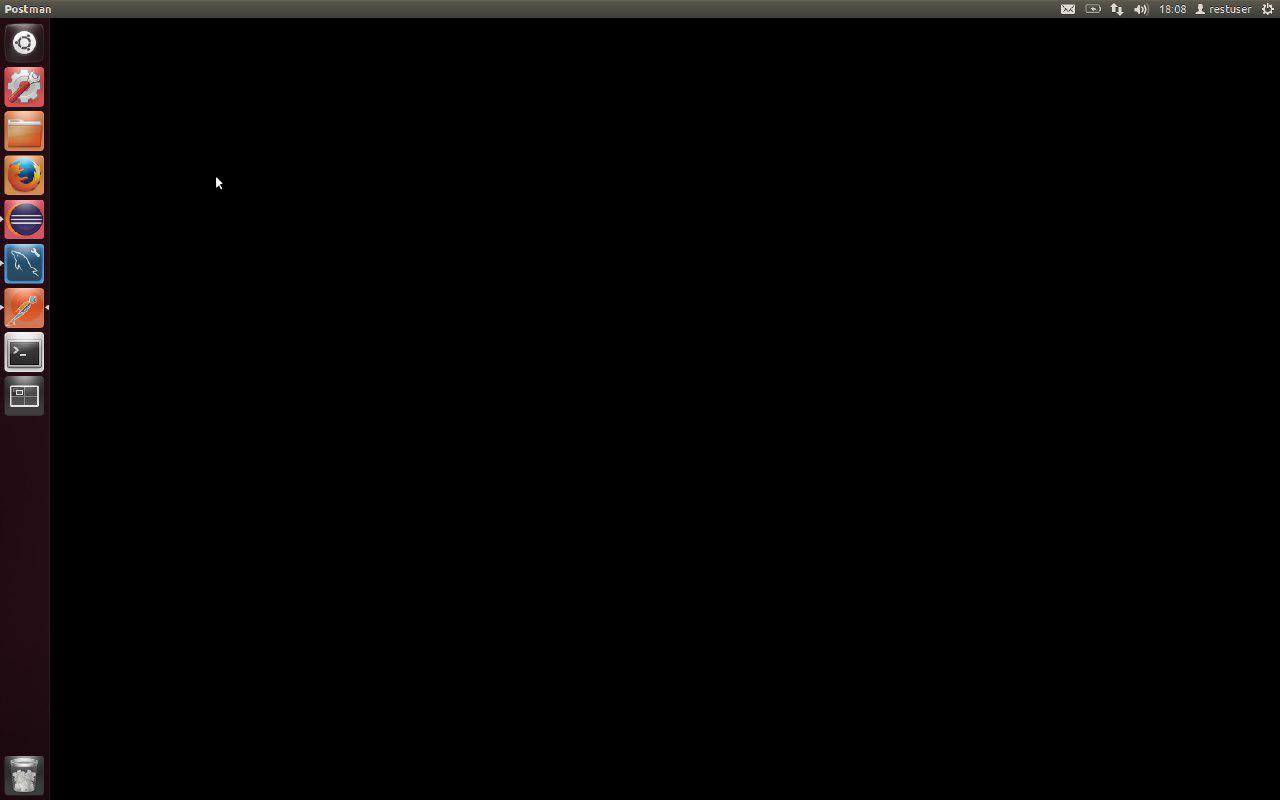
\includegraphics[width=0.45\textwidth]{images/error1.jpg}}
	\subfigure{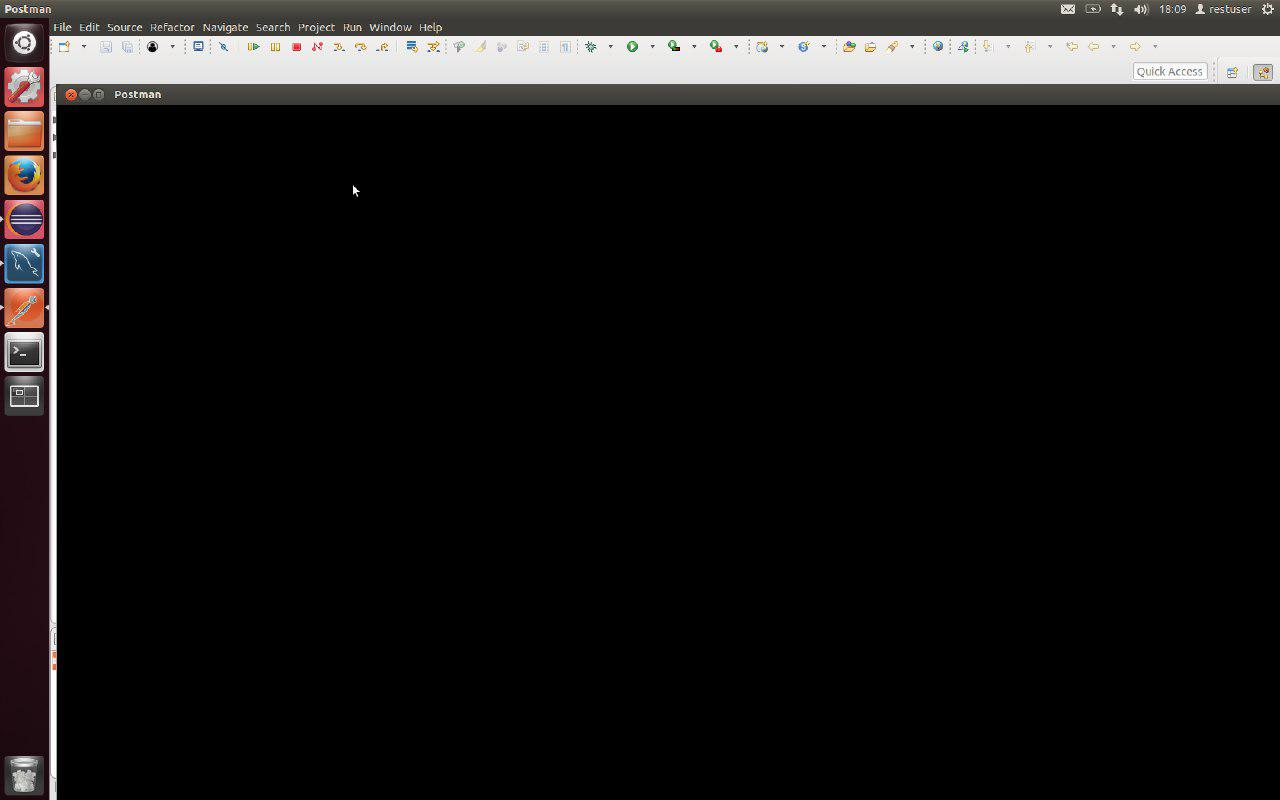
\includegraphics[width=0.45\textwidth]{images/error2.jpg}}
	\caption{Fallo de la aplicación Postman al probar métodos.}
\end{figure}



\end{document}
% --- DOCUMENT ---
